\documentclass[10pt]{article}
\usepackage{float}
\usepackage{amsmath}
\usepackage{paralist}
\usepackage{setspace}
\usepackage{listings}
\usepackage{graphicx}
\usepackage[english]{babel}
\usepackage{geometry}
\usepackage{subcaption}
\usepackage[utf8]{inputenc}
\usepackage{listings}
\usepackage{color}
\usepackage{subcaption}
\usepackage{hyperref}
\usepackage{eurosym}



\begin{document}


\definecolor{mygreen}{rgb}{0,0.6,0}
\definecolor{mygray}{rgb}{0.5,0.5,0.5}
\definecolor{mymauve}{rgb}{0.58,0,0.82}

\lstset{ %
  backgroundcolor=\color{white},   % choose the background color; you must add \usepackage{color} or \usepackage{xcolor}
  basicstyle=\footnotesize,        % the size of the fonts that are used for the code
  breakatwhitespace=false,         % sets if automatic breaks should only happen at whitespace
  breaklines=true,                 % sets automatic line breaking
  captionpos=b,                    % sets the caption-position to bottom
  commentstyle=\color{mygreen},    % comment style
  deletekeywords={...},            % if you want to delete keywords from the given language
  escapeinside={\%*}{*)},          % if you want to add LaTeX within your code
  extendedchars=true,              % lets you use non-ASCII characters; for 8-bits encodings only, does not work with UTF-8
  frame=tb,	                   % adds a frame around the code
  keepspaces=true,                 % keeps spaces in text, useful for keeping indentation of code (possibly needs columns=flexible)
  keywordstyle=\color{blue},       % keyword style
  language=Octave,                 % the language of the code
  otherkeywords={*,...},           % if you want to add more keywords to the set
  numbers=left,                    % where to put the line-numbers; possible values are (none, left, right)
  numbersep=5pt,                   % how far the line-numbers are from the code
  numberstyle=\tiny\color{mygray}, % the style that is used for the line-numbers
  rulecolor=\color{black},         % if not set, the frame-color may be changed on line-breaks within not-black text (e.g. comments (green here))
  showspaces=false,                % show spaces everywhere adding particular underscores; it overrides 'showstringspaces'
  showstringspaces=false,          % underline spaces within strings only
  showtabs=false,                  % show tabs within strings adding particular underscores
  stepnumber=2,                    % the step between two line-numbers. If it's 1, each line will be numbered
  stringstyle=\color{mymauve},     % string literal style
  tabsize=2,	                   % sets default tabsize to 2 spaces
  title=\lstname                   % show the filename of files included with \lstinputlisting; also try caption instead of title
}

\onehalfspacing


\section{CIP 3 - Performance Curves}
\subsection{Introduction}
In this section we analysed the designed turbine under different pitch angles and tip-speed ratios. The design process of a wind turbine differs from turbine to turbine. In order to compare wind turbines non dimensional coefficients are used. These do not depend on factors like size or wind conditions. The most common coefficient is the power coefficient $c_p$. Further we used the torque coefficient $c_q$ and the thrust coefficient $c_t$.
These coefficient are defined as:
\begin{align*}
c_p = \frac{P}{0.5 *\rho A v^3}\hspace{0.5cm}c_t =  \frac{T}{0.5\rho A v^2}\hspace{0.5cm}c_q = \frac{Q}{0.5\rho A v^2*R}\\
\end{align*}
where:\\
$c_p$ = Power coefficient\\
$c_t$ = Thrust coefficient\\
$c_q$ = Torque coefficient\\
$p$   = Power\\
$\rho$ = Density\\
$A$    = Area\\
$v$	   = Windspeed\\
$R$		= Rotorradius

\subsection{WT\_Perf}
To compute the nondimensional parameters a program called WT\_Perf is used. 
WT\_Perf uses blade-element momentum (BEM) theory to predict the performance of wind turbines. \footnote{WT\_Perf\_Users\_guide.pdf}. It also takes different correction algorithms into account, e.g. Prandtl's tip-loss and hub-loss model.
WT\_Perf can be used from the operating system's command prompt. In order to use WT\_Perf  we configured the input file by updating the 'Turbine Data' section and implementing the calculated blade geometry. WT\_Perf also needs the aerodynamic data of the airfoils. We were able to used the provided data here. Last we defined the range of pitch angle and tip-speed ratio according to the tasks of CIP-3. \\
The following code-snippet gives an idea of the input file structure:
\newpage
\begin{lstlisting}
-----  Turbine Data  -----------------------------------------------------------
    3                NumBlade:                  Number of blades.
62.18                RotorRad:                  Rotor radius.
 1.25                HubRad:                    Hub radius. 
 -3.0                PreCone:                   Precone angle, positive downwind.
  5.0                Tilt:                      Shaft tilt.
  0.0                Yaw:                       Yaw error.
  100                HubHt:                     Hub height.
    8                NumSeg:                    Number of blade segments.

  RElm   Twist   Chord  AFfile  PrntElem
 3.808  26.530   6.988	 1	    FALSE
11.424	 9.594   5.407	 1      FALSE
19.040	 2.661   3.832	 1	    FALSE
26.656	-0.866	 2.906	 1	    FALSE
34.272	-1.967   2.171	 2	    FALSE
41.888	-3.354   1.806	 2	    FALSE
49.504	-4.335   1.544	 2	    FALSE
57.120	-5.066   1.348	 2	    FALSE
\end{lstlisting}
\subsection{3.1,3.2}
As already mentioned we configured the input file according to CIP-3. The generated output file contains values for the power coefficient $c_p$, thrust $T$ and torque $Q$.
For task 3.2 we wrote a small python-program which examines the data and plots the results for the three different nondimensional coefficient mentioned in the introduction of CIP-3: $c_p, c_t$ and $c_q$. Since WT\_Perf only writes the power coefficient we had to calculate $c_t$ and $c_q$. Note that the coefficient are functions of $c_t(\lambda), c_q(\lambda)$.
The following figures display the results for $c_p, c_t$ and $c_q$ with a tip-speed ratio $\lambda$ from one to 20 and pitch angles of : 0,5,10,15,20 and 30 degree. The curves are calculated at rated rotor speed (12.59 rpm).

\begin{figure}[H]
\centering
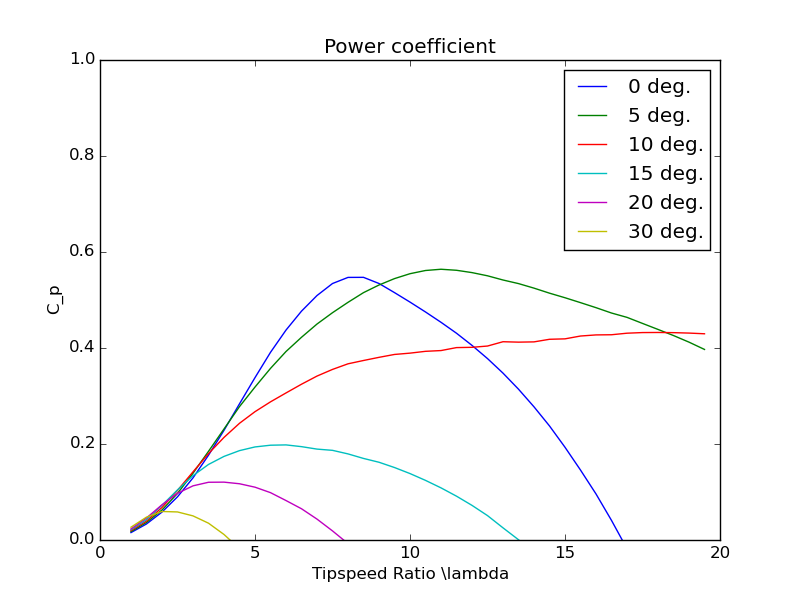
\includegraphics[width=1\linewidth]{../WT_Perf/Output/cp.png}
\caption{Power coefficient}
\label{fig:c-lambda}
\end{figure} 
The $c_p-\lambda$ curve shows different power coefficients at different tip-speeds and pitch-angles. Regarding the maximum for $c_p$ at each curve we identify that they appear at different tip-speed ratios. At pitch angle 5$^\circ$ the maximum $c_p$ is at 0.564 which is very close to the theoretical maximum of 0.592.

\begin{figure}[H]
\centering
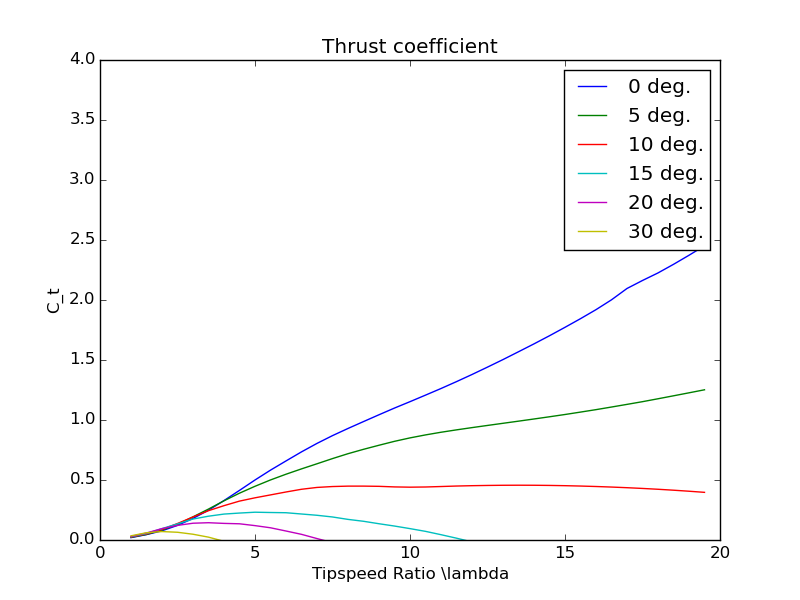
\includegraphics[width=1\linewidth]{../WT_Perf/Output/thrust.png}
\caption{Thrust coefficient}
\label{fig:thrust-coeff}
\end{figure} 
Figure \ref{fig:thrust-coeff} shows the behaviour of the thrust coefficient. 
From 0$^\circ$ to 10$^\circ$ the thrust coefficient reaches high values. For higher pitch angles the resulting thrust coefficient is significantly lower and is equal to zero for higher tip speed ratios. The thrust is directly applied at the tower and can be decreased by increasing the pitch angle.

\begin{figure}[H]
\centering
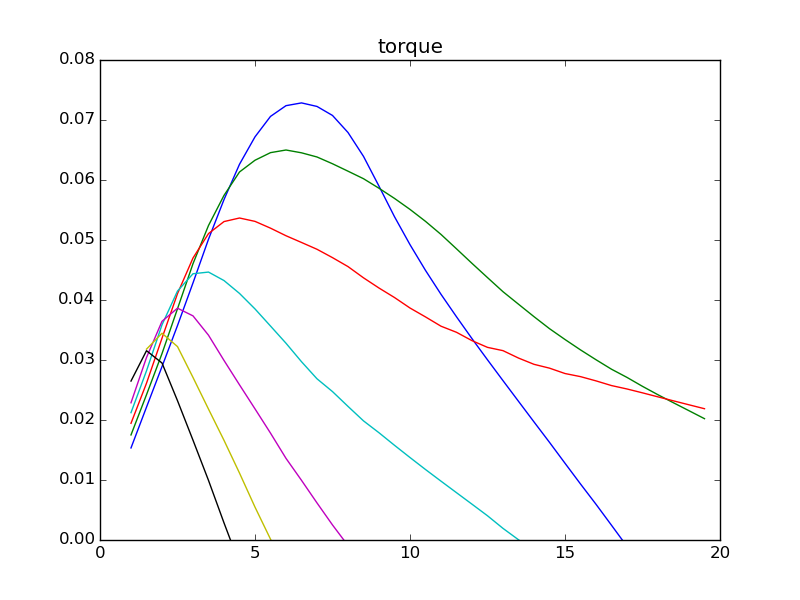
\includegraphics[width=1\linewidth]{../WT_Perf/Output/torque.png}
\caption{Torque coefficient}
\label{fig:torque-coeff}
\end{figure} 
Figure \ref{fig:torque-coeff} shows the torque coefficient for different pitch angles. Compared to the $c_p-\lambda$ the maxima are shifted to the left and decrease with increasing pitch angle.  
\subsection{3.4}
In task 3.4 we were asked to calculate the resulting rotor speed for a rated wind speed of 8 m/s. For the calculation we used our design tip speed ratio:
\begin{align}
\lambda = \frac{\Omega R}{v}\\
n = \frac{60 \lambda v}{2 \pi R} = 10.07 rpm
\end{align}
\subsection{3.5, 3.6}
Again we used WT\_Perf to calculate the resulting operation conditions below rated wind speed. The input parameters are: v = 8 m/s, design top speed ratio $\lambda$ = 8.2 and rotational speed $n$ = 10.07 rpm. The results are shown in the following table:\\

\begin{tabular}{|c |c| c| c| c| c|}
\hline
v & rotor speed & $c_p$ & $c_t$ & $c_q$ & $P$\\
m/s &rpm & - &- &-& kW\\
\hline
8 &10.07&0.544&0.825&0.033& 2054.846\\
\hline
\end{tabular}
Power aus WT\_Perf
\subsection{3.7,3.8}
According to Betz, the wind turbine should be able to extract 7618 kW.
However the rated power of the wind turbine is lower than the power which could be extracted. Therefore pitching is needed. The resulting $c_p$ can be calculated as follows:
\begin{equation}
c_p = \frac{3500000}{0.5 \cdot 1.225 \cdot \pi\cdot  62.18^2 \cdot  12^3} = 0.272
\end{equation}
\subsection{3.9}
\begin{figure}[H]
\centering
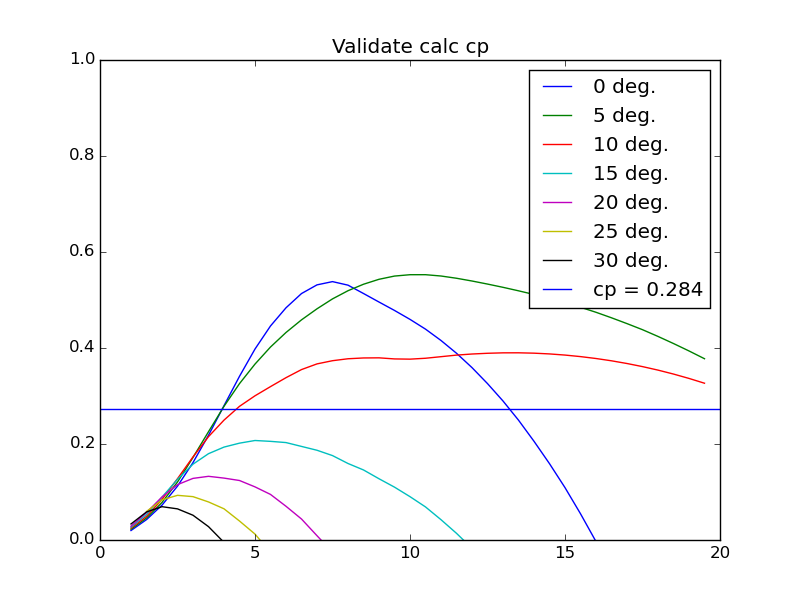
\includegraphics[width=1\linewidth]{../WT_Perf/Output/validated_cp.png}
\caption{Validation of $c_p$}
\label{fig:validate}
The resulting $c_p$ corresponds to a tip speed ratio of 5 with a pitch angle of 10$^\circ$
\end{figure} 
\subsection{3.10}
\begin{align*}
n = \frac{60 \lambda v}{2 \pi R} = 9.21
\end{align*}
\end{document}